\documentclass[journal,12pt,twocolumn]{IEEEtran}
%
\usepackage{setspace}
\usepackage{gensymb}
%\doublespacing
\singlespacing

\usepackage{graphicx}
\usepackage[cmex10]{amsmath}
\usepackage{amsmath,amsthm}
\usepackage{mathrsfs}
\usepackage{txfonts}
\usepackage{stfloats}
\usepackage{bm}
\usepackage{cite}
\usepackage{cases}
\usepackage{subfig}

\usepackage{longtable}
\usepackage{multirow}
\usepackage{commath}
\usepackage{enumitem}
\usepackage{mathtools}
\usepackage{steinmetz}
\usepackage{tikz}
\usepackage{circuitikz}
\usepackage{verbatim}
\usepackage{tfrupee}
\usepackage[breaklinks=true]{hyperref}

\usepackage{tkz-euclide}

\usetikzlibrary{calc,math}
\usepackage{listings}
\usepackage{color}                                            
\usepackage{array}                                            
\usepackage{longtable}                                        
\usepackage{calc}                                             
\usepackage{multirow}                                         
\usepackage{hhline}                                           
\usepackage{ifthen}                                           
\usepackage{lscape}     
\usepackage{multicol}
\usepackage{chngcntr}

\DeclareMathOperator*{\Res}{Res}

\renewcommand\thesection{\arabic{section}}
\renewcommand\thesubsection{\thesection.\arabic{subsection}}
\renewcommand\thesubsubsection{\thesubsection.\arabic{subsubsection}}

\renewcommand\thesectiondis{\arabic{section}}
\renewcommand\thesubsectiondis{\thesectiondis.\arabic{subsection}}
\renewcommand\thesubsubsectiondis{\thesubsectiondis.\arabic{subsubsection}}

\hyphenation{op-tical net-works semi-conduc-tor}
\def\inputGnumericTable{}                                 

\lstset{
	%language=C,
	frame=single, 
	breaklines=true,
	columns=fullflexible
}
\lstset{
	%language=TeX,
	frame=single, 
	breaklines=true
}

\begin{document}
	
	
	\newtheorem{theorem}{Theorem}[section]
	\newtheorem{problem}{Problem}
	\newtheorem{proposition}{Proposition}[section]
	\newtheorem{lemma}{Lemma}[section]
	\newtheorem{corollary}[theorem]{Corollary}
	\newtheorem{example}{Example}[section]
	\newtheorem{definition}[problem]{Definition}
	
	\newcommand{\BEQA}{\begin{eqnarray}}
		\newcommand{\EEQA}{\end{eqnarray}}
	\newcommand{\define}{\stackrel{\triangle}{=}}
	\bibliographystyle{IEEEtran}
	\providecommand{\mbf}{\mathbf}
	\providecommand{\pr}[1]{\ensuremath{\Pr\left(#1\right)}}
	\providecommand{\qfunc}[1]{\ensuremath{Q\left(#1\right)}}
	\providecommand{\sbrak}[1]{\ensuremath{{}\left[#1\right]}}
	\providecommand{\lsbrak}[1]{\ensuremath{{}\left[#1\right.}}
	\providecommand{\rsbrak}[1]{\ensuremath{{}\left.#1\right]}}
	\providecommand{\brak}[1]{\ensuremath{\left(#1\right)}}
	\providecommand{\lbrak}[1]{\ensuremath{\left(#1\right.}}
	\providecommand{\rbrak}[1]{\ensuremath{\left.#1\right)}}
	\providecommand{\cbrak}[1]{\ensuremath{\left\{#1\right\}}}
	\providecommand{\lcbrak}[1]{\ensuremath{\left\{#1\right.}}
	\providecommand{\rcbrak}[1]{\ensuremath{\left.#1\right\}}}
	\theoremstyle{remark}
	\newtheorem{rem}{Remark}
	\newcommand{\sgn}{\mathop{\mathrm{sgn}}}
	\providecommand{\abs}[1]{\(\left\vert#1\right\vert\)}
	\providecommand{\res}[1]{\Res\displaylimits_{#1}} 
	\providecommand{\norm}[1]{\(\left\lVert#1\right\rVert\)}
	%\providecommand{\norm}[1]{\lVert#1\rVert}
	\providecommand{\mtx}[1]{\mathbf{#1}}
	\providecommand{\mean}[1]{E\(\left[ #1 \right]\)}
	\providecommand{\fourier}{\overset{\mathcal{F}}{ \rightleftharpoons}}
	%\providecommand{\hilbert}{\overset{\mathcal{H}}{ \rightleftharpoons}}
	\providecommand{\system}{\overset{\mathcal{H}}{ \longleftrightarrow}}
	%\newcommand{\solution}[2]{\textbf{Solution:}{#1}}
	\newcommand{\solution}{\noindent \textbf{Solution: }}
	\newcommand{\cosec}{\,\text{cosec}\,}
	\providecommand{\dec}[2]{\ensuremath{\overset{#1}{\underset{#2}{\gtrless}}}}
	\newcommand{\myvec}[1]{\ensuremath{\begin{psmallmatrix}#1\end{psmallmatrix}}}
	\newcommand{\mydet}[1]{\ensuremath{\begin{vmatrix}#1\end{vmatrix}}}
	%\numberwithin{equation}{section}
	\numberwithin{equation}{subsection}
	%\numberwithin{problem}{section}
	%\numberwithin{definition}{section}
	\makeatletter
	\@addtoreset{figure}{problem}
	\makeatother
	\let\StandardTheFigure\thefigure
	\let\vec\mathbf
	%\renewcommand{\thefigure}{\theproblem.\arabic{figure}}
	\renewcommand{\thefigure}{\theproblem}
	%\setlist[enumerate,1]{before=\renewcommand\theequation{\theenumi.\arabic{equation}}
	%\counterwithin{equation}{enumi}
	%\renewcommand{\theequation}{\arabic{subsection}.\arabic{equation}}
	\def\putbox#1#2#3{\makebox[0in][l]{\makebox[#1][l]{}\raisebox{\baselineskip}[0in][0in]{\raisebox{#2}[0in][0in]{#3}}}}
	\def\rightbox#1{\makebox[0in][r]{#1}}
	\def\centbox#1{\makebox[0in]{#1}}
	\def\topbox#1{\raisebox{-\baselineskip}[0in][0in]{#1}}
	\def\midbox#1{\raisebox{-0.5\baselineskip}[0in][0in]{#1}}
	\vspace{3cm}
	\title{Assignment 6}
	\author{Addagalla Satyanarayana}
	\maketitle
	\newpage
	%\tableofcontents
	\bigskip
	\renewcommand{\thefigure}{\theenumi}
	\renewcommand{\thetable}{\theenumi}
\begin{abstract}
This document uses the properties of a tangent to a circle
\end{abstract}
Download latex-tikz codes from 
%
\begin{lstlisting}
https://github.com/AddagallaSatyanarayana/AI5106/tree/master/Assignment6/Assignment6.tex
\end{lstlisting}
%
\section{Problem}
Find the length of the tangent from the point $\myvec{7\\4}$ to the circle
\begin{align}
		 \vec{x}^T\vec{x}- \myvec{4 & 6}\vec{x}+12=0\label{eq:1}
\end{align}
\section{Explanation}
The general equation of a second degree can be expressed as :
\begin{align}
	\vec{x}^T\vec{V}\vec{x}+2\vec{u}^T\vec{x}+f=0\label{gen__quad_eqn}
\end{align}
Let the equation of the tangent be
\begin{align}
	\myvec{-m & 1}\vec{x}=c \label{given_line_eq}
\end{align}

\section{Solution}
We know that, for a circle, 
\begin{align}
	\vec{V} = \vec{I}  \\
	\vec{c} = -\vec{u}
\end{align}
Comparing the equation \eqref{eq:1} and \eqref{gen__quad_eqn}
we get
\begin{align}
	\vec{u}&=\myvec{-2 \\ -3}, f=12 \\
	\vec{c}&=\myvec{2 \\ 3}
\end{align} 

The normal vector to the line is obtained as 
\begin{align}
	\vec{n} = \vec{q} + \vec{u} \label{eq1}\\
	\vec{q} = \vec{n} - \vec{u}
\end{align}

Comparing the equation \eqref{given_line_eq} 
\begin{align}
	\vec{n} &= \myvec{-m &1}^T
\end{align}
Given
\begin{align}
	 \vec{u}&=\myvec{-2 \\ -3}\\
\implies	 \vec{q} &= \myvec{-m+2 \\ 4}\label{eq:2}
\end{align}
The point q also satisfies the equation of the circle at \eqref{eq:1}
\begin{align}
	\vec{q}^T\vec{q}+2\vec{u}^T\vec{q}+f=0\\
	(\vec{n} -\vec{u})^T(\vec{n} -\vec{u})+2\vec{u}^T(\vec{n} -\vec{u}) +f =0\\
	\norm{\vec{n}}^2 - \vec{n}^T\vec{u}-\vec{u}^T\vec{n}+\norm{\vec{u}}^2+2\vec{u}^T\vec{n}- 2\norm{\vec{u}}^2+f=0\\
	\norm{\vec{n}}^2 -\norm{\vec{u}}^2+f=0\\
	m^2+1-13+12=0\\
	m^2=0\\
	m=0\label{eq:3}
\end{align}
Simplying \eqref{eq:3} and \eqref{eq:2} we get
\begin{align}
	\vec{q} &= \myvec{2 \\ 4}
\end{align}

Let $\vec{p} =\myvec{7 \\ 4}$
The length of tangent is 
\begin{align}
	\norm{p-q}&= \sqrt{(7-2)^2 + (4-4)^2}\\
	&=\sqrt{25}\\
	&=5
\end{align}
 \begin{figure}[!htbp]
 	\centering
 	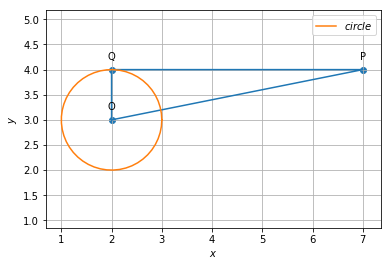
\includegraphics[width =\columnwidth]{circle.png}
 	\caption{Perpendicular Line }
 	\label{fig:1}
 \end{figure}	

\end{document}